\chapter{Implementation}\label{C:impl}

\section{Front End}  %this needs a better title, badly.

web application, written using javascript, css and html5.

Figure \ref{overview} shows an overview of the Honeynet dataset. In a column to the left, we have some controls for the visualisation. To the right, taking up the majority of space is a timeline visualisation of logged data.  
<Explain basic interactions here, related back to functional and nonfunctional requirements. >
<explain why features were cut, here or design?>

Both date boxes are linked to datepicker tools, which allow for chosing a date from a calendar, and setting time through sliders. These values may be freely edited without reloading data. The Jump to dates button will trigger a reload of data. 
Binlength (Immediately below date controls) allows chosing the length of each timebin. the dropdown controls units (from seconds to years), while the textbox accepts a number of units.
<Complete detailed description>
\begin{figure}[h!]
\fbox{\parbox[b]{.99\linewidth}{
\centering 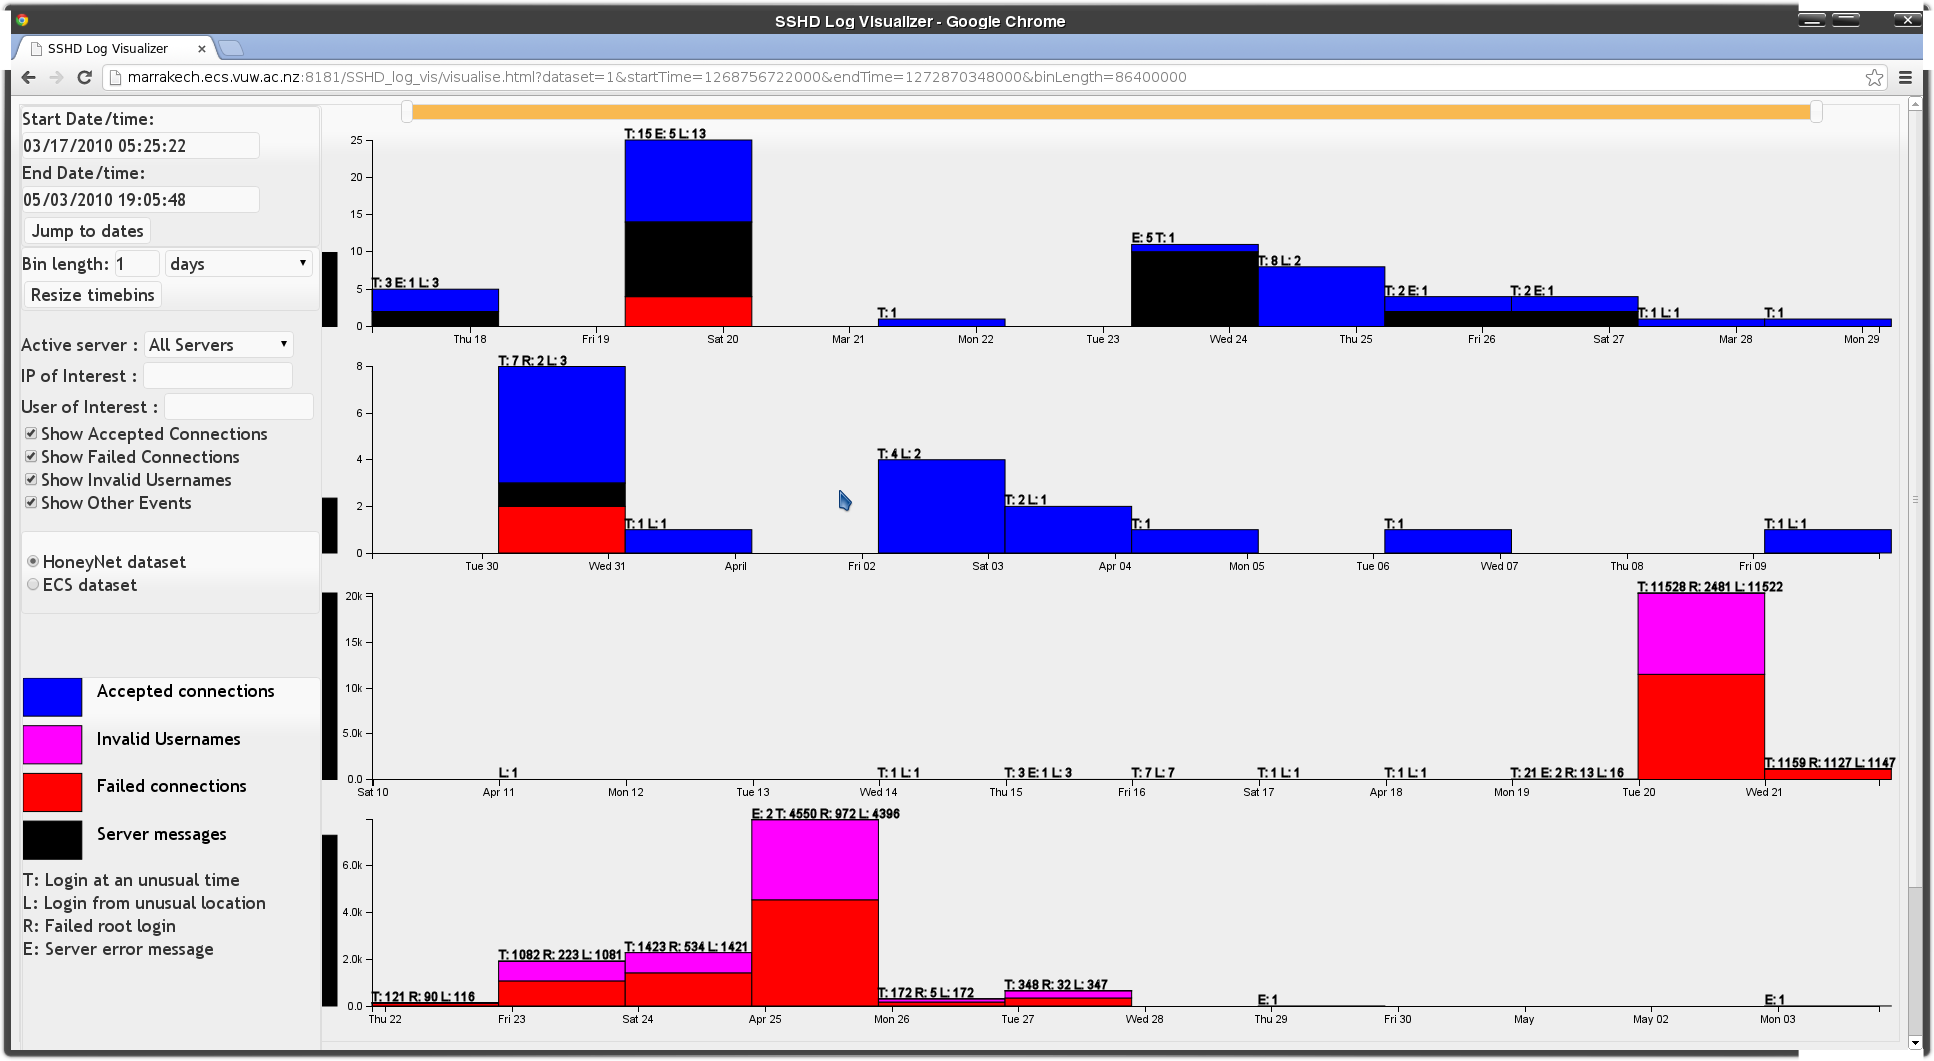
\includegraphics[scale=0.43,  angle=270]{screenshots/overview.png}
}}
\caption{\protect\label{overview}Tool showing overview of the honeynet dataset (\ref{data})}
\end{figure}


\section{Database}
Not a heck of a lot to discuss here, other than why RDBMS is kinda irrelevant to server thanks to jOOQ. (except sqlite, not suitable for multiuser environments.)
also discuss performance issues with GeoIp data. (inability to use index for range queries of the form const between column A, and column B), Use of geospatial extensions to resolve this.

\section{Parser}

Very simpleminded parser. This would require a significant rewrite to move datastores, as the database schema is encoded in the format of statements used to insert data. 

Currently built for RDBMS system.

Also handles location and time clustering, using a simple online algorithm in conjunction with the datastore. very primitive and simpleminded algorithms, but capable of processing an infinite stream of data (albeit in infinite time). This simple streaming approach was taken as it's not possible to determine in the general case how long a logfile may be. Use cases also call for ability to read data as written by the SSH demon. 

\section{Server}

Design of server side code and functions remains to be carried out, though I plan to perform the majority of data processing server side, due to concerns about javascript and browser performance when hundreds of thousands to millions of elements are being manipulated. 

architecture. two layer model. data access layer, and client communication layer. 
could be refactored into a three layer model, to allow expansion beyond web clients. 
\begin{itemize}
\item{Data access layer. Responsible for fetching data from the underlying datastore. easily replaced to communicate with different kind of datastore. Takes values from client communication layer, returns lists of matching log entries.}
\item{Client Communication layer. Responsible for aggregating data returned by the data access layer, and building HTTP responses from the aggregated data. Including JSON translation.}
\end{itemize}
<include description of tomcat + servlet architecture here.>

data access layer has a defined interface, with methods for fetching data to satisfy each type of request.
\begin{itemize}
\item{Fetch log lines - used to fetch all log lines between a given pair of timestamps, with optional filters on username, server, and source IP}
\item{Fetch start and end times - used to fetch the timestamps of the first and last events in the datastore}
\item{Fetch all server names - used to fetch a list of every server name known to the datastore}
\end{itemize}

The underlying implementation for these methods currently targets RDBMS systems, though so long as the interface is maintained, this could be replaced with any other datastore.

4 types of request that may be made of the server
\begin{itemize}
\item{Request aggregated events between given timestamps, and optional filters on username, server, and source IP}
\item{Request raw events between given timestamps, and optional filters on username, server, and source IP}
\item{Request start and end timestamps}
\item{Request list of all servernames}
\end{itemize}

All request types are implemented as independent servlets within the web application. Each servlet has no shared state, so parallelizes easily within the tomcat framework. Connection pooling is implemented to assist in performance where multiple users may be requesting data. Concurrent read/write issues are the responsibility of the underlying datasource.

The first two request types use the same interface to the datasource, but have differing post processing applied. raw does not do any agreggation, simply converts the data into JSON format and embeds in the HTTP response. aggregated collects statistics about all events which fall in that time period, statistics are transmitted in JSON format as payload of HTTP response.
Why have aggregated request? nonfunctional requirements - performance and data hiding. aggregation done serverside due to bandwidth and memory requirements, this operation could involve processing millions of nodes for larger logs. This is unreasonable to send across the network in raw form, due to size and space requirements. Server has resources to do aggregation. 
some room for refactoring, this could be split into two layers
however the processing is quite simple, and only done for this one request type, so a data analysis layer was omitted.

\section{Security Concerns}
Rewrite to explain security model, including server choices that allow for defence in depth.
As I'm building the tool as a client server model, accessed through the browser
there are several security concerns to be considered in a deployment of the system.
The database will contain a significant amount of privileged information about network security
such as machine names and addresses, valid account names, and authentication methods used in the system.

This data would be extremely useful to malicious users or outside intruders. 
This leads to a need to ensure that access to this database is controlled through a robust authentication system.
Ideally the web server hosting the tool should not be accessible to the outside world at all. Within the organisation's private network access should be restricted tightly to only those users with a definite need to have access. 
Secured connections must be used for all communication between client and server to limit the opportunity for malicious individuals to snoop on the data in transit.

Security of the serverside code will be considered from the beginning of the design and implementation process
as this code must be able to resist any malicious access attempts. Through input sanitation and bounds checking should serve to close the majority of possible vulnerabilities.

Client side code contains no data, and so is significantly less critical to secure, as the database systems should deny access without valid credentials. Ideally host based authentication could be used. However, implementing a robust access control scheme does not fit within the scope of this project, and will be left for future development.


\section{Testing}
Automated testing of user interfaces remains problematic, with many tools suffering from severe fragility where UI layout is modified. In most testing libraries, mous interaction is recorded at test design, then played back artificially on execution, This causes severe fragility as if a control or button moves the recorded mouse movements will miss the button, causing test failures. Further research is needed to find a testing library suitable for testing, however the test automation tool created by Dojo appears useful \cite{dojo2013test}. - automated testing not used. heavy use of in browser dev tools and debugger. manual testing. 

\begin{figure}[tbh]
\fbox{\parbox[b]{.99\linewidth}{
\vskip 0.5cm
\centering 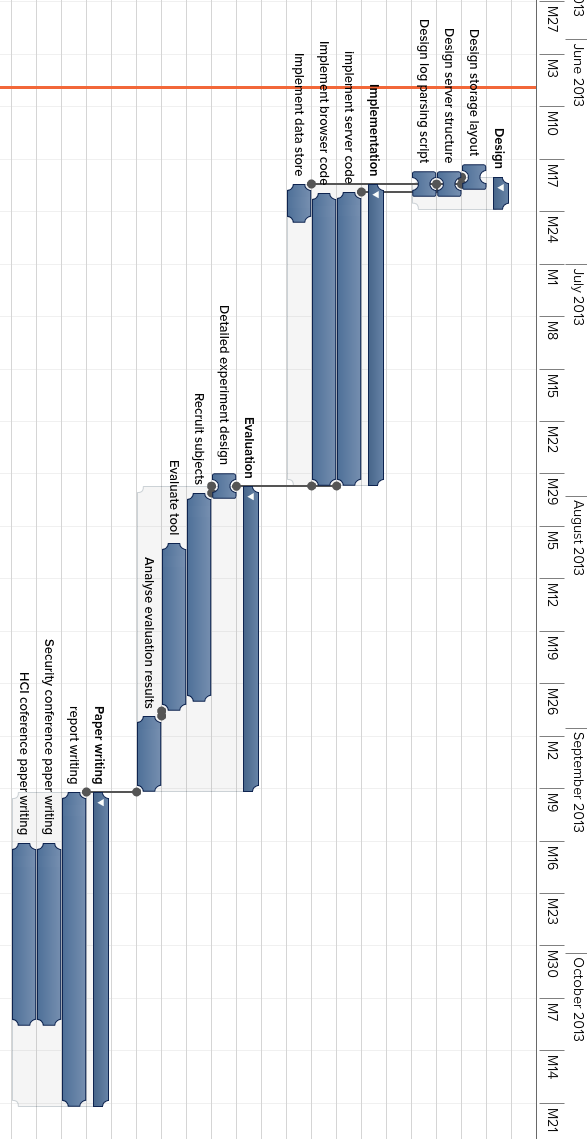
\includegraphics[scale=0.75]{gantt.png}
\vskip 0.5cm}}
\caption{\protect\label{gantt}Gantt chart showing breakdown of future work into major sections. The design group is all sub day tasks.}
\end{figure}